\documentclass[11pt,a4paper]{article}  % Déclare la classe du document.

\newcommand{\chaptermark}[2]{\og #2 \fg{} (#1)} % ligne uniquement pour éviter une erreur en cas d'article
\include{../1ere-preambule}

\usepackage{epic}   % extension et simplification de  l'environnement picture
\usepackage{graphicx}    % permet d'inclure des graphique externe dans un document
\usepackage{arydshln}   %permet d'avoir des lignes en pointillés
\let\dx\undefined
\usepackage{bardiag}

\newcommand{\lignes}[1]{
	\setlength{\unitlength}{1mm}
	\vskip 0,4cm\noindent
	\multido{\i=0+1}{#1}{%
		\noindent
		\begin{picture}(150,5)
			\linethickness{0,005mm}
			\put(-5,0){\dashline{1}(175,5)(5,5)}
		\end{picture}\vskip 0,001cm
	}
	\vskip 0cm
}

\rhead{\textcolor{red}{Correction - DS n$^{\circ}01$ - Statistiques - 18/11/2024}}

\newcommand{\va}[1]{\lvert \ #1 \ \rvert}
\newcommand{\vaf}[1]{\left\lvert \ #1\  \right\rvert}

\begin{document}
	\graphicspath{{images/}}
	
	\begin{center}
		
		
		\fbox{
			\begin{minipage}[]{15cm}
				\begin{center}
					\LARGE{\rule{0.5cm}{0pt}\rule[-0.25cm]{0pt}{0.9cm}
						\textcolor{red}{Correction - DS n$^{\circ}01$ \\
						Statistiques} 
					}
				\end{center}
			\end{minipage}
		}
	\end{center}

\begin{center}\textbf{1h20min - Barème indicatif}\end{center}
\begin{center}\textbf{Les élèves avec un tier-temps ne traitent pas les questions avec  le symbole \ding{46}}\end{center}
\begin{center}\textbf{Calculatrice autorisée.\\Les résultats devront être justifiés (à l'aide de calcul ou de propriétés).}\end{center}


\exerciceDS{ - (5 points)}
%environ 15-20 min
Le gérant d'une librairie spécialisée dans la bande dessinée souhaite réaliser un bilan annuel de ses ventes. Il a regroupé certaines informations dans le tableau suivant:\\
\begin{tabular}{|Xc|Xc|Xc|Xc|Xc|}
	\cline { 2 - 5 } \multicolumn{1}{c|}{} & BD européenne & Comics & Manga & Total \\
	\hline 1er semestre & 13 100 & 16 700 & \textcolor{red}{22 700} & 52 500 \\
	\hline 2nd semestre & 9 100 & \textcolor{red}{4 100} & 9 300 &  \textcolor{red}{22 500} \\
	\hline Total & \textcolor{red}{22 200}  & \textcolor{red}{20 800}  & \textcolor{red}{32 000} & 75 000 \\
	\hline
\end{tabular}
\begin{enumMet}
	\item Interpréter les nombres 75 000, 52 500 et 9 300 dans le contexte de cet exercice.
	\begin{corrBox}
		75 000 correspond au chiffre d'affaire annuel total de ses ventes. \quad \bareme{1}\\
		52 500 correspond au chiffre d'affaire du 1er semestre. \quad \bareme{1}\\
		9 300 correspond au chiffre d'affaire de la vente de manga au 2ème semestre. \quad \bareme{1}
	\end{corrBox}
	\item Compléter ce tableau. \quad \bareme{2}
\end{enumMet}

%\exerciceDS{ - (5 points)}
%Le tableau suivant correspond au bilan journalier des ventes de tickets dans un cinéma.\\
%\begin{tabular}{|Xc|Xc|Xc|Xc|}
%	\cline { 2 - 4 } \multicolumn{1}{c|}{} & Femmes & Hommes & Total \\
%	\hline Enfants (- de 18 ans) & 220 & 260 & 480 \\
%	\hline Adultes & 320 & 550 & 870 \\
%	\hline Seniors (+ de 65 ans) & 420 & 630 & 1050 \\
%	\hline Total & 960 & 1440 & 2400 \\
%	\hline
%\end{tabular}
%\begin{enumMet}
%	\item \begin{enumMet}
%		\item Donner l'effectif total de cette population.
%		\item Quel est l'effectif marginal des femmes ?
%	\end{enumMet}
%	\item Quel est l'effectif des hommes adultes venus au cinéma ce jour-là?
%	\item Interpréter dans le contexte de l'exercice :
%	\begin{enumMet}
%		\item le nombre 480 ;
%		\item le nombre 420.
%	\end{enumMet}
%\end{enumMet}

\exerciceDS{  \ding{46} - (2 points)}
Le service d'intendance met à jour les fiches des 150 élèves de première générale d'un lycée. 95 élèves sont externes, 31 élèves participent au dispositif \guillemets{petit déjeuner} et 48 élèves sont demi-pensionnaires et ne participent pas à ce dispositif. Compléter le tableau ci-dessous.\\

\begin{tabular}{|Xc|Xc|Xc|Xc|}
	\cline { 2 - 4 } \multicolumn{1}{c|}{} & Demi-pensionnaire & Externe & Total \\
	\hline Participe au dispositif &  \textcolor{red}{7} & \textcolor{red}{24}  & \textcolor{red}{31}  \\
	\hline Ne participe pas au dispositif &  \textcolor{red}{48} & \textcolor{red}{71}  & \textcolor{red}{119}  \\
	\hline Total & \textcolor{red}{55}  & \textcolor{red}{95}  & \textcolor{red}{150}  \\
	\hline
\end{tabular}

\exerciceDS{  - (4 points)}
Le tableau ci-dessous donne l'origine de l'électricité qui a été consommée en France le dimanche 11 décembre 2022 de 13 h à 14 h selon RTE.

\begin{tabular}{|Xc|Xc|Xc|}
	\hline Origine & \begin{tabular}{Xc} 
		Consommation \\
		(en Mégawatt)
	\end{tabular} & Angle \\
	\hline Import & 5 646 & \textcolor{red}{$31\degree$}\\
	\hline Fossile & 9 122 & \textcolor{red}{$49\degree$} \\
	\hline Renouvelable & 11 150 & \textcolor{red}{$61\degree$}\\
	\hline Nucléaire & 40 368 & \textcolor{red}{$219\degree$}\\
	\hline Total & 66 286 & $360^\circ$\\
	\hline
\end{tabular}

\ \\
Compléter le tableau et représenter ces données par un diagramme circulaire.

\ \\

\Stat[Qualitatif,Graphique,Angle,Rayon=1.5cm, ListeCouleurs={Turquoise
	,LightSteelBlue,PaleGreen,GreenYellow}]{%
	Import/31,%
	Fossile/49,%
	Renouvelable/61,%
	Nucléaire/219}

\exerciceDS{ - (6 points)}
Le diagramme circulaire ci-dessous donne la répartition des 17700 surfeurs licenciés en France pour la saison 2019-2020.

\begin{minipage}[c]{0.4\linewidth}
	\begin{center}
		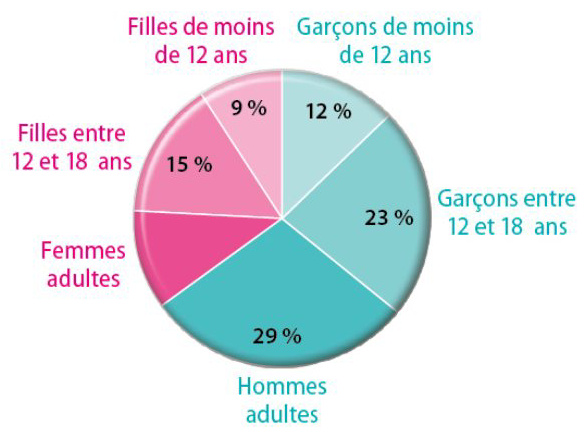
\includegraphics[scale=0.45]{DS_img01}
	\end{center}
\end{minipage} \hfill
\begin{minipage}[c]{0.6\linewidth}
	\begin{enumMet}
		\item La Fédération Française de Surf annonce que la majorité des licenciés sont des jeunes (moins de 18 ans). A-t-elle raison ? Justifier. \quad \bareme{2}\\
		\begin{corrBox}
			$15+9+12+23=59>50$. La FFS a raison. $59\%$ des licenciés sont des jeunes.
		\end{corrBox}
		\item Quel pourcentage des licenciés représentent les femmes adultes ? \quad \bareme{1}\\
		\begin{corrBox}
			$100-(15+9+12+23+29)=12\%$
		\end{corrBox}
		\item Calculer le nombre de garçons de moins de 12 ans.	 \quad \bareme{1} \corr{$\dfrac{12}{100}\times17700=2124$}
		\item Établir un tableau croisé d'effectifs décrivant la répartition des licenciés selon leur genre et leur âge. \quad \bareme{2} \\
	\end{enumMet}
\end{minipage}

\begin{corrBox}
	\begin{tabular}{|Xc|Xc|Xc|Xc|Xc|}
		\hline Tranche d'âge & $<12$ ans & $12-18$ ans & adultes & Total \\
		\hline Hommes & 2124 & 4071 & 5133& 11328\\
		\hline Femme & 1593 & 2655 & 2124 & 6372\\
		\hline Total & 3717 & 6726 & 7257 & 17700\\
		\hline
	\end{tabular}\\
\end{corrBox}



%\newpage


\exerciceDS{ - (5 points)}
Le tableau ci-dessous représente le pourcentage de différents usages d'Internet selon la tranche d'âge entre 2017 et 2021.\\
\begin{tabular}{|Xc|Xc|Xc|Xc|}
	\hline Tranche d'âge & $16-24$ ans & $25-64$ ans & $65-74$ ans \\
	\hline Journaux & 63 & 61 & 41 \\
	\hline Jeux en ligne ou téléchargés & 53 & 28 & 13 \\
	\hline Radios en ligne, musique en streaming & 82 & 51 & 18 \\
	\hline Vidéos ou télévision sur Internet & 89 & 55 & 25 \\
	\hline Voyages et hébergement & 41 & 46 & 30 \\
	\hline
\end{tabular}\\
\ \\
Représenter les données du tableau à l'aide d'un diagramme en barres.

\ \\
%this is the way to redefine styles
\newpsstyle{mytickstyle}{linewidth=1pt,linecolor=blue}
%
%\newpage
\def\onecol{Peach}
\def\twocol{ProcessBlue}
\def\thirdcol{YellowGreen}
\renewcommand{\betweenticks}{5}
\renewcommand{\shownumbers}{1}
\renewcommand{\numbercolor}{\Large\black\bf}
\newpsstyle{diagframestyle}{linewidth=1pt,linecolor=black}
%\newpsstyle{levellinestyle}{linewidth=0.2pt,linecolor=blue}
\newpsstyle{barstyle}{linewidth=2pt,linecolor=black}
\bardiagrambegin{20}{90}{2.5cm}{1}{4}{0.8cm}{0.1cm}
\barspergroup{3}
\drawlevellines
\baritem{Journeaux}{63}{\onecol}
\subbaritem{}{61}{\twocol}
\subbaritem{}{41}{\thirdcol}
\baritem{Jeux}{53}{\onecol}
\subbaritem{}{28}{\twocol}
\subbaritem{}{13}{\thirdcol}
\baritem{Radio}{82}{\onecol}
\subbaritem{}{51}{\twocol}
\subbaritem{}{18}{\thirdcol}
\baritem{Vidéo}{89}{\onecol}
\subbaritem{}{55}{\twocol}
\subbaritem{}{25}{\thirdcol}
\baritem{Voyages}{41}{\onecol}
\subbaritem{}{46}{\twocol} 
\subbaritem{}{30}{\thirdcol} 
%
% we can call
%\diagLegendoptions{yellow}{yellow}{0.0pt}
% to produce a legend with yellow background with yellow frame
%
\diagLegendbegin{15.5}{88}{4}
\diagLegenditem{16-24 ans}{\onecol}
\diagLegenditem{25-64 ans}{\twocol}
\diagLegenditem{65-74 ans}{\thirdcol}
\diagLegendend
\bardiagramend{\large Usages d'internet}{\large pourcentage}

\newpage

\exerciceDS{ Lancers francs au basketball - (8 points)}

Line et Basil s'affrontent aux lancers francs.
Le gagnant est celui qui aura le meilleur taux de succès sur l'ensemble de ses tentatives. Voici les résultats obtenus lors de deux manches.

\begin{tabular}{|Xc|Xc|Xc|Xc|Xc|}
	\cline { 2 - 5 }
	\multicolumn{1}{l|}{ } & \multicolumn{2}{c}{ Manche 1 } & \multicolumn{2}{c}{ Manche 2 }  \\
	\cline { 2 - 5 } \multicolumn{1}{l|}{ }  & Basil & Line & Basil & Line \\
	\hline Succès & 30 & 10 & 3 & 4 \\
	\hline Échecs & 20 & 6 & 17 & 16 \\
	\hline
\end{tabular}\\


On souhaite déterminer qui a gagné à partir de ces deux séries de lancers.
\begin{enumMet}
	\item \begin{enumMet}
		\item Calculer le taux de succès de chacun d'entre eux lors de la manche 1. \quad \bareme{1}
		\begin{corrBox}
			Basil : taux$=\dfrac{30}{50}=60\%$
			
			Line : taux$=\dfrac{10}{16}=62,5\%$
		\end{corrBox}
		\item Calculer de même le taux de succès de chacun lors de la manche 2 . \quad \bareme{1}
		\begin{corrBox}
			Basil : taux$=\dfrac{3}{20}=15\%$
			
			Line : taux$=\dfrac{4}{20}=20\%$
		\end{corrBox}
		\item Qui a remporté chacune des manches? \quad \bareme{1}
		\begin{corrBox}
			C'est Line qui a gagné les 2 manches.	
		\end{corrBox}
	\end{enumMet}
	\item \begin{enumMet}
		\item \ding{46} Compléter le tableau suivant sur l'ensemble des deux manches. \quad \bareme{2}
		
		\begin{tabular}{|l|l|l|}
			\cline { 2 - 3 } \multicolumn{1}{c|}{} & Basil & Line \\
			\hline Succès & \textcolor{red}{33} & \textcolor{red}{14}\\
			\hline Échecs & \textcolor{red}{37} & \textcolor{red}{22}\\
			\hline
		\end{tabular}
		\item \ding{46} Calculer le taux de succès de chacun sur l'ensemble des deux manches. \quad \bareme{1}
		\begin{corrBox}
			Basil : taux$=\dfrac{33}{70}\approx47,1\%$
			
			Line : taux$=\dfrac{14}{36}\approx 38,8\%$
		\end{corrBox}
		\item \ding{46} Qui a gagné sur le cumul des deux manches \quad \bareme{1}
		\begin{corrBox}
			C'est Basil qui gagne sur le cumul des 2 manches.	
		\end{corrBox}
	\end{enumMet}
	\item \ding{46} Que peut-on observer ? Expliquer. \quad \bareme{1}
	\begin{corrBox}
		En faisant le cumul, la situation s'inverse. Cela s'explique car lors de la première manche, leur \% de réussite est très similaire alors que Basil a fait beaucoup plus de lancers alors que pour la deuxième manche (raté pour les 2) ils ont lancés le même nombre de ballons. 
	\end{corrBox}
\end{enumMet}

\end{document}

